\chapter{Introduction}%
\label{chap:introduction}
\textit{This chapter narrows the broad field of robotics down to a largely unsolved problem. For that problem the state of the art methods are presented, and their shortcomings are highlighted. \Cref{sec:research_question} addresses the current gap in research with the main and sub research questions. A largely unsolved problem is then narrowed down to the scope of this thesis in problem description,~\cref{sec:problem_description}. The chapter finishes by presenting all upcoming chapters in the report structure,~\cref{sec:report_structure}.\bs}

\todo[inline]{Corrado: All my feedback latest feedback from this chapter}

% What's Purpose: The following issues are presented:
% - introduce 3 topics
% - joint-configuration space
% - multiple modes of dynamics, piecewise analytic
% - there are not much state-of-the-art methods, but these are them
% - backward search / backward induction

% What's Purpose: introduce 3 topics
For robots, it remains a hard problem to navigate and act in new, unseen environments. It can be motivated that this is due to many challenges that the robot has to overcome. In this thesis such challenges are categorised into 3 topics, namely: \textbf{learning object dynamics}, \textbf{\ac{NAMO}} and \textbf{nonprehensile manipulation planning}.
\todo[inline]{motivation should be in this order, learning namo, pushing}
\todo[inline]{can you use this: 
Combining learning, driving and pushing can improve the driving and pushing skills of the robot. Learning is crucial for unforeseen environments, for example during space exploration. Non-prehensile pushing compared to prehensile pushing saves weight, and for a robot with a gripper the ability for nonprehensile pushing comes in handy when the gripper is already in use, for example when a robot relocates a package with its gripper, it encounters a blocked path by an unknown object. Blocked paths and changing environments often coincide, such as a fallen package in a warehouse spilling fluid on the floor, with learning the robot can account for the slippery floor. Finally learning may improve single actions, but it may also improve long-term action planning.\bs}
Robots can face unseen environments during for example space exploration or rescue missions in collapsed buildings, but also in more everyday robot applications. So can an unfamiliar environment emerge from a familiar environment due to some unforeseen change the robot is not aware of. An example is a leakage that changes the friction coefficient between the floor and everything that stands on it. Another example are supermarkets, due to the presents of people in the supermarket the environment changes, providing a slightly new environment for robots that operate in them. Learning abilities allow robots to operate in completely new enironments and improve robots to adapt to environmental changes. Research into approaches tackling the 3 topics just described can be split into two categories. The bulk falls into the category hierarchical approaches~\cite{kaelbling_hierarchical_2011,scholz_navigation_2016,krontiris_dealing_2015}. The remainder falls in category locally optimal approaches ~\cite{vega-brown_asymptotically_2020,sabbaghnovin_optimal_2016,novin_dynamic_2018,sabbaghnovin_model_2021}. Both approaches are elaborated upon later in this chapter, first a number of problems are highlighted.\bs

% What's Purpose: joint configuration space
The first problem is emerges from the combination of robots performing \ac{NAMO} \textit{and} pushing tasks. Imagine a robot that can drive and push objects around in its environment, the robot is then tasked to relocate an number of objects. A solution to such a task consist of a number of drive and a number of push actions, where every drive or push action acquires a path from start to target location. Finding a path  is known as a \textit{motion} or \textit{manipulation planning problem} and requires a configuration space. Configuration space can be described as a $n$-dimensional space related to a single object, where $n$ is the number of degrees of freedom for that single object. The workspace obstacles are mapped to configuration space obstacles that make up obstacle space. The remainder of obstacle space subtracted from configuration space is free space, in which the object can move freely. For every object in the environment a configuration space can be constructed. A \textit{joint configuration space} emerges when the robot's configuration space is augmented with the configuration space of every object. For example, if the configuration space for both robot and objects consist of position $x$, $y$ and orientation $\theta$ around the $z$ axis (thus $n=3$) then the joint configuration space is $3m$-dimensional, where $m$ is the number of objects in the environment including the robot. Thus the dimensionality of the joint configuration space grows linearly with the number of object in the robot environment, also known as the \textit{curse of dimensionality}. Going back to the robot tasked with relocating a number of objects. For a solution a path is sought from the current configuration of the environment, a point in the joint configuration space to a target point in joint configuration space where all objects a at their target position. Conventional motion planners cannot efficientely find a path because of the enormity of the joint configuration space. The enormity can be described by the following analysation. Drive actions put the robot on a new location, push actions put an object at a new location, both influencing the configuration spaces of all other an object in the environment. Thus future planning is influenced by the actions taken now. Another analysation that describes the hugeness of the joint configuration space are unspecified target positions. During relocation of objects, other objects might be present in the environment. No target location is specified for such objects, whilst they could be essential to relocate in order to put the objects with target positions at their target positions. Consider a blocked corridor, the blocking object needs to be pushed to free the path but the target location of the blocking object is unspecified, as long as the robot can drive through the corridor unhindered. The target point in joint configuration space is thus not unique.\bs

% What's Purpose: multiple modes of dynamics, piecewise analytic
\paragraph{Challenges}
Finding a optimal solution to a \ac{NAMO} and pushing task requires a search in the joint configuration space. Apart from the fact that the joint configuration space grows ridiculously fast, there is another problem. The joint configuration space is \textit{piecewise-analytic}, which is now explained. Drive and push actions are translated to the joint configuration space as subspaces. A certain subspace of the joint configuration space is assigned to robot driving and other subspace is assigned to robot pushing. These different subspaces in joint configuration space are called different modes of dynamics. In the driving mode of dynamics a set of driving constraints must be respected, the pushing mode has a set of push constraints that must be respected. Such constraints originate from e.g.~the robot being nonholonomic, geometry and weight distribution of objects and friction coefficient between the robot and objects. Because there is a discontinuity in the constraints the joint configuration space is a piecewise-analytic. Motion planners have great difficulty crossing the boundary from one mode of dynamics to another mode of dynamcis~\cite{vega-brown_asymptotically_2020}.\bs

As mentioned before finding an optimal solution to a \ac{NAMO} and pushing task requires a search in joint configuration space. If the problem is simplified by taking out relocating objects to new positions from the task, a purely \ac{NAMO} problem is what remains. If the problem is simplified even further, by assuming every object to be a unmovable obstacle, the problem falls in the category of \ac{NP-hard} problems because, it is equivalent to the piano mover's problem which is known to be \ac{NP-hard}~\cite{reif_motion_1985}.\\
\todo[inline]{look at this part with papie}
Problems in class P have a solution which can be found in polynomial time, problems in \ac{NP} are problems for which a solution cannot found in polynomial time. For problems in \ac{NP}, when provided with a solution, verifying that the solution is indeed a valid solution can be done in polynomial time. \ac{NP-hard} problems are a class of problems which are at least as hard as the hardest problems in \ac{NP}. Problems that are \ac{NP-hard} do not have to be elements of NP. They may not even be decidable~\cite{pokharel_computational_2020}. This thesis or other recent studies in the references do not attempt to find an optimal solution. Instead, they provide a solution whilst guaranteeing properties such as near-optimality or probabilistic completeness. We conclude that the \ac{NAMO} problem combined with relocating objects to target positions fall in the category of \ac{NP-hard} problems because it can be reduced to the piano's mover problem.\bs

The last problem that is introduced it the uncertainty of actions in unknown evironments. Planning an action sequence with limited or no environment knowledge inevitably leads to unfeasible action sequences, such as pushing unmovable obstacles. Updating the environment knowledge and replanning the action sequence is the cure to the uncertainty introduced by a lack of environment knowledge. Unfeasible action sequences are time and resources lost, additionally it can lead task that become unfeasible. For example, a pushing robot end up pushing an object into a dead due to an action sequence planned with limited environment info. Now that the object is in a stuck position the task has become unfeasible.\bs

To summerise, the main challenge is to find an action sequence for a given task to relocate objects that consists of push and drive actions. To find such action sequence a path from start configuration in joint configuration space to a desired target configuration in the joint configuration space, where all specified objects are at their specified target position. The emerged challenges are the enormity of the joint configuration space, the different modes of dynamics that make the joint configuration space piecewise-analytic, and lastly the uncertainty introduced by the lack of prior environment knowledge.\bs

\todo[inline]{FROM HERE LOCALLY OPTIMAL APROACHES}
\paragraph{State of the art Methods}
% What's Purpose: there are not much state-of-the-art methods, but these are them
Now the state of the art methods are discussed that can be categorised in two categories. Locally optimal and hierarchical approaches, first locally optimal approaches are discussed. As has been indicated in the previous paragraph, finding a path in the joint configuration space cannot computationally be found in reasonable time (orders of magnitude slower than real-time, with no guarantees if no path exists). Only by leveraging simplifications applied to the joint configuration space a search can be performed, such as considering probabilistic simplified environment~\cite{vandenberg_path_2009}, considering a single manipulation action~\cite{berenson_manipulation_2009}, discretization~\cite{sabbaghnovin_optimal_2016} or a heuristic function combined with a time horizon~\cite{sabbaghnovin_optimal_2016}. Such techniques prevent searching in configurations relatively far from the current configuration. Local optimality guarantees can be given and real-time implementations have been shown.\bs

The most relevant locally optimal approach is presented by \citeauthor{sabbaghnovin_model_2021} she presents a optimal motion planner that avoids obstacles in the workspace and respects kinematic and dynamic constraints of a robot arm~\cite{sabbaghnovin_optimal_2016}. Examples of the motion planner are provided using a 3- and 4- \ac{DOF} planar robot arm~\cite{sabbaghnovin_optimal_2016}. Sampling in the joint configuration space is simplified using discritisation (by disjunctive programming) of the joint configuration space and by using a receding horizon. The disjunctive programming concept is applied for converting the continuous problem of path planning into a discrete form. In other words, a continuous path is made equivalent to some points with equal time distances which represent the entire path~\cite{sabbaghnovin_optimal_2016}. After discretisation the joint configuration space remains huge, thus a search is performed close to the current configuration by combining a heuristic function with a receding horizon concept. A specially developt heuristic function points \textit{toward} the target configuration, the planner then plans between the current configuration and a point toward the target configuration for a predetermined time horizon. The concept of a receding horizon is used to obtain the optimal path for every time step in the time horizon, but apply only the first term and repreating this process until the end-effector meets the final position~\cite{sabbaghnovin_optimal_2016}.\bs

The optimal motion planner~\cite{sabbaghnovin_optimal_2016} is then converted toward path planning for a nonholonomic mobile robot with a gripper~\cite{novin_dynamic_2018}. With the 4-fingered gripper the robot can grasp legged objects such as chairs or walkers. The targeted workspace is a hospital, where the robot is tasked with handing walkers (or other legged objects) to patients to lower the number falling patients. The variety of legged objects motivates an object model learning module that learns dynamic parameters from experimental data with a legged objects. The dynamic parameters are learned using an Bayasian regression model~\cite{scholz_navigation_2016}, an \ac{MPC} controller then tracks the path and compensates for modeling errors. A key contribution is that the planner can decide to regrasp one of the objects legs to improve path tracking.\bs

Real world experiments show the effectiveness of Novin's locally optimal approach~\cite{sabbaghnovin_model_2021}. She has presented a manipulation planning framework focussed on moving legged objects in which the robot has to choose between which leg to push or pull. The framework can operate in real time, and the local optimality have been shown~\cite{sabbaghnovin_model_2021}. From the 3 topics that this thesis focusses on, \citeauthor{sabbaghnovin_model_2021} includes learning and prehensile manipulation of objects to target positions, missing only the \ac{NAMO} problem because a path is assumed to be free during object manipulation. Because Novin uses a gripper to manipulate objects, her research falls into the category of prehensile manipulation. Prehensile manipulation is considered easier in comparison with nonprehensile manipulation because it is harder to disconnect a gripped object.\bs

\todo[inline]{FROM HERE HIERARCHICAL APPRAOCHES}
The second approach to find a path in joint configuration space are classified as hierarchical approaches~\cite{vega-brown_asymptotically_2020,kaelbling_hierarchical_2011,scholz_navigation_2016,wang_affordancebased_2020} that can be described as follows. A hierarchical structure generally consists of a high-level and a low-level component. The high-level task planner has an extended time horizon which includes several atomic actions and their sequencing. Whilst a low level controller acts to accomplish a single action that acts in a single mode of dynamics (e.g.~drive toward object, push object), by sending input signals toward the robot actuators. The high-level planner has a prediction horizon consisting of an action sequence, a long prediction horizon compared to the low-level planner whose prediction horizon is maximal for a single action.\bs

The most relevant hierarchical approach is presented by \citeauthor{scholz_navigation_2016} he presents a planner for the \ac{NAMO} problem that can handle environments with under-specified object dynamics~\cite{scholz_navigation_2016}. The robot's workspace if split into various free space regions can be connected by manipulating the object that seperates these regions. The manipulation action is uncertain, because objects have constraints that the robot has to learn e.g. a table has a leg that only rotates, but cannot translate. An \ac{MDP} is choosen as a graph-based structure, where the nodes represent a free space region and objects seperating the regions are edges in the \ac{MDP}. Finding a solution for the \ac{MDP}, leads to an action sequence consisting of a number of drive an object manipulation actions to eventually drive the robot toward a target position. The under-specified object dynamics introduce uncertainty in object manipulation. During action execution object constraints are captured with a physics-based reinforcement learning framework that results in improving manipulation planning when replanning is triggered.\bs

\citeauthor{scholz_navigation_2016} presented a \ac{NAMO} planner that makes use of a hierarchical \ac{MDP} combined with a learning framework, resulting in online learning of the under-specified object dynamamics. The methods effectiveness in learning and driving toward a target location has been shown by an implementation on a real robot. From the 3 topics that this thesis focusses on, \citeauthor{scholz_navigation_2016} includes learning and the \ac{NAMO} problem, missing only push manipulation toward target locations. By not including manipulation of objects to target positions \citeauthor{scholz_navigation_2016} is able to find a global path without running into high dimensional spaces. In other words, by driving only the robot toward a target location a global path will encounter objects only once. By running into objects only once the manipulation of an object does not affect the feasiblity of the global path, hence the simplification.\bs


Both local optimal and hierarchical approaches have been discussed, both having their advantages and disadvantages. Local optimal approaches can theoretically converge to a global optimal plan. To avoid the curse of dimensionality simplifications must be used to sample the joint configuration space in order to be computionally feasible, such simplifications determine the quality of solutions found. Hierarchical structures generally provide solutions which are computationally efficient but are hierarchical, meaning the solutions found are the best feasible solutions in the task hierarchy they search. The quality of the solution depends on the hierarchy which is typically hand-coded and domain-specific~\cite{vega-brown_asymptotically_2020}. The most relevant work for local optimal~\cite{sabbaghnovin_model_2021} and hierarchical~\cite{scholz_navigation_2016} approaches are discussed. What they both have in common, both combine 2 of the 3 topics (learning, the \ac{NAMO} problem, object manipulation toward target positions). Note both relevant works focus on prehensile manipulation, whilst this thesis focusses on nonprehensile manipulation. Individually a considerable amount of research is done on these topics (\ac{NAMO}~\cite{wang_affordancebased_2020,lavalle_planning_2006,elbanhawi_samplingbased_2014,kingston_samplingbased_2018,chen_fast_2018,ellis_navigation_2022}, nonprehensile manipulation planning~\cite{arruda_uncertainty_2017,mericli_pushmanipulation_2015,toussaint_sequenceofconstraints_2022,stuber_let_2020,stuber_featurebased_2018,bauza_dataefficient_2018}, learning object dynamics~\cite{seegmiller_vehicle_2013,cong_selfadapting_2020}), combining two topics recieves little attention by scientific community, and combining all three topics (to the best of my search) not at all. \Cref{table:sota_and_3_topics} shows multiple relevant literature and which portion of the 3 topics they include in their research.\bs

\begin{table}[H]
  \centering
  \rowcolors{2}{white}{myEvenLighterColor}
  \begin{tabular}{P{2.5cm} P{1.5cm} P{1.8cm} P{1.8cm} P{1.8cm} p{1.9cm}}
    Author & Citation & Learns\newline object\newline dynamics & \ac{NAMO} & Specify object target positions & Object\newline Manipulation\\ 
    \citeauthor{sabbaghnovin_model_2021} &\cite{sabbaghnovin_model_2021} & \cmark& \xmark& \cmark& grasp-push grasp-pull\\
    \citeauthor{scholz_navigation_2016} &\cite{scholz_navigation_2016} & \cmark& \cmark& \xmark& graph-push grasp-pull\\
    \citeauthor{krontiris_dealing_2015} &\cite{krontiris_dealing_2015} & \xmark& \cmark& \cmark& gripping\\
    \citeauthor{wang_affordancebased_2020} &\cite{wang_affordancebased_2020} & \cmark& \cmark& \xmark& pushing\\
    \citeauthor{vega-brown_asymptotically_2020} &\cite{vega-brown_asymptotically_2020} & \xmark& \cmark& \cmark& gripping\\
    \citeauthor{ellis_navigation_2022} &\cite{ellis_navigation_2022} & \cmark& \cmark& \xmark& pushing\\
    Groote & proposed solution &  \cmark& \cmark& \cmark& pushing\\
  \end{tabular}
  \caption{Overview of 3 topics in recent literature and their object manipulation, where \textit{grasp-push} and \textit{grasp-pull} refer to prehensile push and pull manipulation, \textit{gripped} refers to fully gripping and lifting objects for manipulation, \textit{pushing} refers to nonprehensile push manipulation.}%
  \label{table:sota_and_3_topics}
\end{table}

\textbf{The main contribution of this thesis is to combine all three topics.} A backward search in the joint configuration space is performed \todo[inline]{introduce the next paragraph}\bs

% What's Purpose: backward search / backward induction
\paragraph{Backward Search}
This thesis proposes a method where the robot should learn robot and object dynamics by interaction, and perform motion and manipulation planning whilst facing a wide variety of objects, tasks and environments. The 3 topics (\ac{NAMO}, nonprehensile manipulation planning and learning system models) are bundled together with a technique known as \textbf{backward induction} also known as \textbf{backward tracing} or \textbf{backward search} (this thesis will refer to this technique with the term backward search).\todo[inline]{Marijn: strange sentence} The proposed method in this thesis and \citeauthor{sabbaghnovin_model_2021} proposed method solve comparable problems using different techniques, allowing for easy comparison between the results of \citeauthor{sabbaghnovin_model_2021} and the results from the proposed method in this thesis.\bs
\todo[inline]{Martijn : explain backward induction, backward tracing and provide references}

\section{Research Question}%
\label{sec:research_question}
To investigate the effect of learning on action selection and on action planning the following research questions have been selected.\bs

\textbf{Main research question:}
\begin{center}%
\label{researchquestion:main}
\large
How do learned objects' system models improve global task planning\\for a robot with nonprehensible manipulation abilities over time?
\end{center}

The main research question is split into two smaller more detailed subquestions. Essentially the first research subquestion asks \quotes{how does the proposed method work?}, which allows to explain the proposed method. The second research subquestion essentially asks: \quotes{How does it compare to similar existing methods?}, allowing to compare the proposed methods with existing state-of-the-art methods by comparing their results.\bs

\textbf{Research subquestion:}
\begin{enumerate}
    \item\label{researchsubquestion:does_it_work} Can the proposed method combine learning and planning for push en drive applications with a technique known as backward search~\cite{krontiris_dealing_2015}?
    \item\label{researchsubquestion:does_it_compare} How does learning system models and remembering interactions compare to only learning system models? And, how does the proposed method compare against the state of the art?
\end{enumerate}

Answering the research subquestions provides a solid base to answer the main research question. The main research question is aimed to test robot abilities in a new environment, and track improvement in that a new environment. Some questions which come up are: Will the robot prefer specific strategies for certain objects? How much improvement will a robot make with some experience? Will the robot converge to a preferred strategy for an object, and will it converge to the same strategy again if its memory is wiped.\bs

\section{Problem Description}%
\label{sec:problem_description}
\todo[inline]{Martijn: So, why at all was a 3D environment selected?}
To answer the research questions, tests will be performed in a robot environment. A simple environment is desired because that will simplify testing, yet the robot environment should represent many real-world environments in which robots operate. For the environment, a flat ground plane is selected, since many mobile robots operate in a workspace with a flat floor, such as a supermarket, warehouse or distribution centre. The robots to test should be flat robots, which lowers the chance of tipping over. A 3-dimensional environment is selected, but with a flat floor and a flat robot can be treated as a 2-dimensional problem because the robot and objects can only change position over $x$ and $y$ axis ($xy$ plane parallel to the ground plane) and rotate around the $z$ axis (perpendicular to the ground plane).\bs

Let's start with defining the environment.\\Let the tuple $\left\langle \text{Origin}, \text{Ground Plane}, \text{Ob}, E \right\rangle$ fully define a robot environment where:\bs

\par\smallskip\noindent
\centerline{\begin{minipage}{0.8\textwidth}
\begin{enumerate}
  \item[Origin] Static point in the environment with a $x$-, $y$- and $z$-axis. Any point in the environment has a linear and an angular position and velocity with respect to the origin \vspace{0.5\baselineskip}
 \item[Ground Plane] A flat plane parallel with the Origin's $x$- and $y$- axis. Objects cannot pass through the ground plane and meet sliding friction when sliding over the ground plane. \vspace{0.5\baselineskip}
 \item[Ob] A set of objects, $\text{Ob} = (obst_1, obst_2, obst_3, \dots, obst_i)$ with $i>1$, an object is a 3-dimensional body with shape and uniformly distributed mass. Examples of objects are given in \cref{fig:example_objects}. \vspace{0.5\baselineskip}
  \item[$E$] A set of motion equations describing the behaviour of objects such as gravity, interaction with the ground plane or interaction with other objects. The motion equations are equivalent to the true dynamics. \vspace{0.5\baselineskip}
\end{enumerate}
\end{minipage}}
\par\smallskip

   \todo[inline]{Martijn: Why do you call them "obst"? This seems related to the woord Obstacle, not Object.}
   \todo[inline]{Marijn: why do you say i>1?}

\todo[inline]{Martijn: what does this mean, "equivalent to the true dynamics"?}
A state consists of the linear and angular position and velocity of a point with respect to the environment's origin.\bs
\todo[inline]{Martijn: points cannot have angular positions. Also, I don't think that states are properties of points, rather of systems (such as the robot or an object or the whole system including the robot and all objects).}

Formally, a \textbf{state}, $s_{id}(k)$ is a tuple of $\left\langle pos_x(k), pos_y(k), pos_\theta(k), vel_x(k), vel_y(k), vel_\theta(k)\right\rangle$\\ where $pos_x, pos_y, vel_x, vel_y, vel_\theta \in \mathbb{R}, \quad  pos_\theta \in [0, 2\pi)$, \quad $k$ indicates the time step and can be removed for simplicity if the state remains constant for all $k$.\\
\todo[inline]{Martijn: wath is id?}
\todo[inline]{Martijn: actually, in the introduction you very frequently use the concept "configuration space" and later in 1.2.3 you go back to configuration space, so it is odd that you do not define that space here, but state space instead.}
\todo[inline]{Martijn: actually, in the introduction you very frequently use the concept "configuration space" and later in 1.2.3 you go back to configuration space, so it is odd that you do not define that space here, but state space instead.kk}

\subsection{Task Specification}%
\label{subsec:task}
The research questions want to investigate the effect of learning system models and monitor the effect of learned knowledge over time. Thus the robot needs an incentive to learn object properties, and interactions with the objects in its environment, otherwise it would simply remain standing still in its initial location. Therefore the robot is asked to complete a task. A task is defined as a subset of all objects with associated target states:\bs
\[\text{task} = \left\langle Obst_{task}, S_{targets} \right\rangle\]

where $Obst_{task} = (obst_1, obst_2, obst_3, \dots, obst_k) \subset Ob$, $S_{target} = (s_1, s_2, s_3, \dots s_k)$ and $k>0$\bs

\todo[inline]{martijn: as you define it here, these target states seem to include the angle theta as well as the velocities. Are you sure that your results (which are not in the document yet) will show that all of these states will be reached through the robot's pushing? I suspect that your results will only show that the objects will reach target positions (x,y), not target angles and certainly not any target velocities other than zero. If my suspicion is correct, you need to more accurately define your target configuration here.}

\todo[inline]{Martijn: why k>0? (and why does this differ from the equally contested statement earlier regarding i>1)?o}

A task is completed when the robot manages to push every object to its targets position within a specified error margin.

\subsection{Assumptions}%
\label{subsec:assumptions}
A complex robot environment is not required to answer the research questions. Therefore influences other than the robots are neglected, some real-world dynamics which are generally negligible are neglected, a workaround is found to measure uncertain properties and the objects in the environment will not tip over. To simplify the pushing and learning problem, several assumptions are taken, which are now listed.\bs
\todo[inline]{Martijn: I don't really understand what you are trying to say here.}

\begin{assumption*}%
\label{assumption:closed_world}
\textbf{Closed-World Assumption:} Objects are manipulated, directly or indirectly only by the robot. Objects cannot be manipulated by influences from outside the environment.
\end{assumption*}\bs

\begin{assumption*}%
\label{assumption:quasi_static}
\textbf{Quasi-Static Assumption:} Velocities are small enough that inertial forces are negligible~\cite{stuber_let_2020}.
\end{assumption*}\bs
\todo[inline]{Gijs: Remove the quasi static assumption, it only provides head paint. Martijn: whether or not inertial forces can be neglected is not (solely) determined by how small velocities are, so the "argument" that you provide here is incorrect., Martijn: If you really completely embrace a quasi-static assumption, then I doubt that velocities can still be considered part of the state of the robot. k}

\begin{assumption*}%
\label{assumption:perfect_object_sensor}
\textbf{Perfect Object Sensor Assumption:} the robot has full access to the poses and geometry of all objects in the environment at all times.
\end{assumption*}\bs

\begin{assumption*}%
\label{assumption:order_does_not_matter}
\textbf{Tasks are Commutative Assumption:} Tasks consist of multiple objects with specified target positions. The order in which objects are pushed toward their target position is commutative.
\end{assumption*}\bs

\begin{assumption*}%
\label{assumption:no_tipping}
\textbf{Objects do not tip over Assumption:} Movable objects slide if pushed.
\end{assumption*}\bs

The assumptions taken serve to simplify the problem of task completion. Note that in \cref{sec:future_work} insight is given to remove all assumptions except the quasi-static assumption. By removing assumptions completing tasks becomes a harder problem, but a more realistic problem closer to real-world applications.\bs

Assumptions might have certain implications, which are now listed. The \hyperref[assumption:closed_world]{\textbf{closed-world assumption}} implies that objects untouched by the robot and with zero velocity component remain at the same position. Completed subtasks are therefore assumed to be completed for all times after completion time.\bs

The \hyperref[assumption:quasi_static]{\textbf{quasi-static assumption}} allows neglecting complex dynamics, which in many cases are negligible. To ensure that complex dynamics do not become significant during testing, a maximum robot speed or acceleration is enforced.\bs
\todo[inline]{Martijn: I assume that the document will somewhere contain the exact calculation for determining the value of these upper limits. Gijs: Truely, this has to be included. }

The \hyperref[assumption:perfect_object_sensor]{\textbf{perfect object sensor assumption}} simplifies a sensor setup, it prevents Lidar-, camera setups and tracking setups with aruco or other motion capture markers. The existence of a single perfect measurement wipes away the need to combine measurements from multiple sources with sensor fusion algorithms, such as Kalman filtering \cite{verhaegen_filtering_2007}.\bs

Certain tasks are only feasible if performed in a certain order (e.g. the Tower of Hanoi), the \hyperref[assumption:order_does_not_matter]{\textbf{tasks are commutative assumption}} allows focusing only on a single subtask since it does not affect the completion or feasibility of other subtasks.\bs

The \hyperref[assumption:no_tipping]{\textbf{objects do not tip over assumption}} ensures that objects do not tip over and suddenly have vastly different dynamics. In practice, objects will not be higher than the minimum width of the object, and spheres are excluded since rolling essentially is tipping.
\todo[inline]{Martijn: this height limit does not necessarily guarantee that objects will not tip over; this also depends on the friction coefficient with the floor, and the point of application of (push) contact forces.}

\paragraph{Robot and Objects, an Example}
To get a sense of what the robots and the objects look like, see the two robots that are used during testing in \cref{fig:example_robots}. And among many different objects, two example objects are displayed in \cref{fig:example_objects}.

\todo[inline]{Martijn: what about the orientation (angle)? You do list angle as part of the state, so I do expect the angle to be controlled. Gijs: make clear that the pointrobot has not angle, that is only for the boxer robot.}
\begin{figure}[H]
    \centering
    \begin{subfigure}{.5\textwidth}
    \centering
    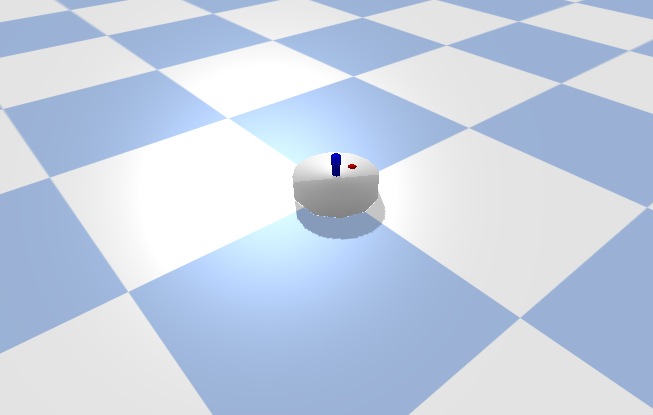
\includegraphics[width=0.8\textwidth]{figures/point_robot.png}
    \caption{The holonomic point robot\\the 2 velocity inputs drive the robot in $x$ and in $y$ direction}%
    \label{subfig:example_point_robot}
    \end{subfigure}%
    \begin{subfigure}{.5\textwidth}
    \centering
    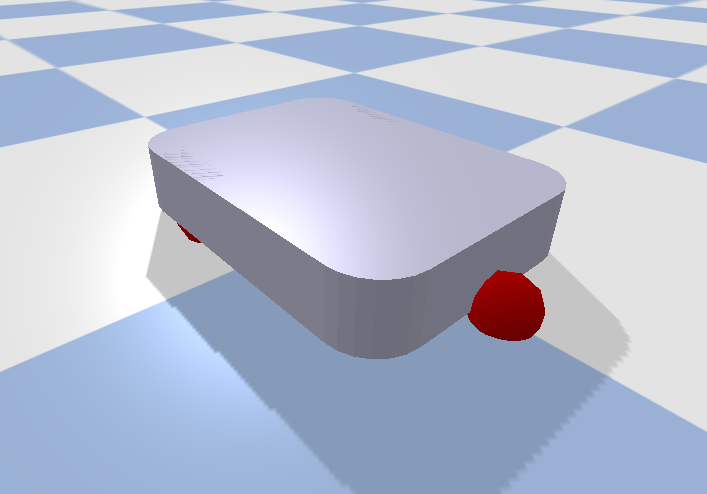
\includegraphics[width=0.8\textwidth]{figures/boxer_robot.png}
    \caption{The nonholonomic boxer robot\\the first velocity input drives the robot forward/backward\\the second rotates the robot}%
    \label{subfig:example_boxer_robot}
    \end{subfigure}%
    \caption{Robots used for testing the proposed method}%
    \label{fig:example_robots}
\end{figure}

\begin{figure}[H]
    \centering
    \begin{subfigure}{.5\textwidth}
    \centering
    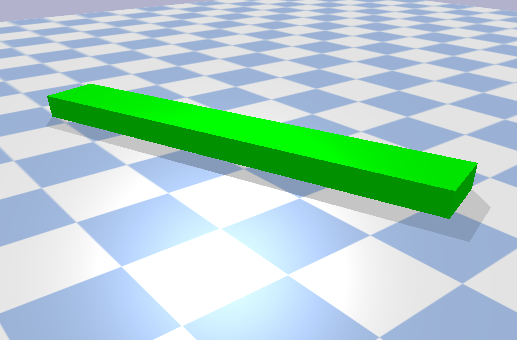
\includegraphics[width=0.8\textwidth]{figures/box_object.png}
    \caption{A box object}
    \end{subfigure}%
    \begin{subfigure}{.5\textwidth}
    \centering
    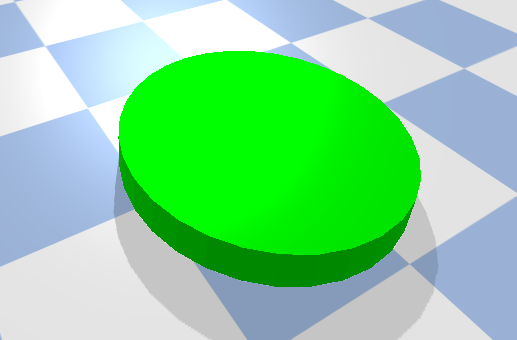
\includegraphics[width=0.8\textwidth]{figures/cylinder_object.png}
    \caption{A cylinder object}
    \end{subfigure}%
    \caption{Various objects in the robot environment}%
    \label{fig:example_objects}
\end{figure}

For complete environments with accompanying tasks, see~\cref{chap:results}.\bs


\section{Report Structure}%
\label{sec:report_structure}
\todo[inline]{Create the report structure when the report structure does not change anymore}



The proposed solution will essentially avoid searching directly in the joint configuration space and will search in subspaces of the joint configuration space where only a single mode of dynamics is present. Subchallenges that emerge are system identification, control methods, estimating path existence, motion and manipulation planning. These subchallenges will be properly introduced and elaborated on in \cref{chap:hgraph_and_kgraph}.\bs



